%%%%%%%%%%%%%%%
\task{Падающие стулья}
\begin{itemize}
\itA Стул с пятнадцатью ножками упал с лестницы из пяти ступенек и сломал одну ножку. Потом он упал с лестницы из десяти ступенек и сломал три ножки. Сколько ножек он сломает, упав с лестницы из 20 ступенек?

\itB В кафе стоит $n$ четырёхногих стульев. Ночью в кафе заходит мальчик Вася и начинает вслепую подпиливать стульям ножки. С утра стул упадёт под посетителем, если у него останутся неподпиленными меньше трёх ножек. Сколько ножек нужно подпилить Васе, чтобы с утра как минимум $m$ посетителей кафе гарантированно упали?

\itC В кафе $n$ четырёхногих стульев. Стул падает, если у него меньше трёх целых ножек. У мальчиков Васи и Пети есть две пилы, и они изобретают себе игру. Мальчики уже сошлись на том, что первым ходит Петя, а проигрывает тот, после чьего хода упадёт первый стул. Осталось выбрать возможное число перепиливаний за ход для каждого из них. Пусть за каждый ход Петя перепиливает не менее чем $a_1$ и не более чем $b_1$ ножек, Вася — от $a_2$ до $b_2$ ножек. Числа $a_1$ и $a_2$ могут быть равны нулю или единице, а числа $b_1$ и $b_2$ — $m$ или $m-1$, $m<n$, но при этом обязательно $b_1 \ne b_2$. Сколько игр удовлетворяет этим условиям, и кто из мальчиков выиграет в каждой из них?
\end{itemize}
%%%%%%%%%%%%%%%

%%%%%%%%%%%%%%%
\task{Детский сад}
\begin{itemize}
\itA В детском саду 10 детей рисуют 10 рисунков за 20 минут. Как долго 50 детей будут рисовать 50 рисунков? Как долго $d$ детей будут рисовать $r$ рисунков?

\itB Детсадовцам Вове и Диме выдали по обручу — обруч представляет собой диск радиусом $r_1$, из которого вырезан круг радиуса $r_2$, $r_2<r_1$. Мальчики стали клеить пластилин на выданные им обручи. За минуту Вова наращивал сантиметр пластилина на внешнем краю обруча, а Дима — сантиметр пластилина на внутреннем его краю. У кого из мальчиков площадь обруча росла быстрее?

\itC В медпункт детского сада пришло четверо детей. У медсестры есть двухчашечные весы без гирь, и она хочет расположить детей по весу. Сколько взвешиваний ей для этого нужно сделать? Как ей производить взвешивания?
\end{itemize}
%%%%%%%%%%%%%%%

%%%%%%%%%%%%%%%
\task{Числа, выписанные на доску}
\begin{itemize}
\itA Коля в свой День рождения выписал на доску наименьшее число, дважды содержащее все цифры от 0 до 9 и делящееся на 72. Выпишите и вы это число!

\itB А Оля записала на доску числа от 1 до 121 и теперь занимается следующим: стирает с доски числа $a$ и $b$, записывая вместо них разность вида $a-2b$ либо $b-2a$. Могло ли в конце на доске остаться единственное число — ноль?

\itC На доску выписаны $n$ чисел. Доказать, что одно из них или сумма нескольких рядом стоящих чисел непременно делится на $n$.
\end{itemize}
%%%%%%%%%%%%%%%

%%%%%%%%%%%%%%%
\task{Линии и сетки}
\begin{itemize}
\itA В стол вбиты 26 гвоздиков так, как показано на рисунке 5. Расстояние между соседними~— 1 сантиметр. Помогите Любе пропустить по столу нитку длиной 25 сантиметров от гвоздика $A$ к гвоздику $B$ так, чтобы она касалась каждого гвоздика.

\itB На клетчатой бумаге начертили прямоугольник размерами $a$ на $b$, по линиям сетки. Может ли проведённая на том же листе прямая пройти по $a+b$ клеткам в составе этого прямоугольника?

\itC Среди треугольников с данным основанием $l$ и данным периметром $P$ найти треугольник с максимальной площадью.
\end{itemize}

\begin{center}
  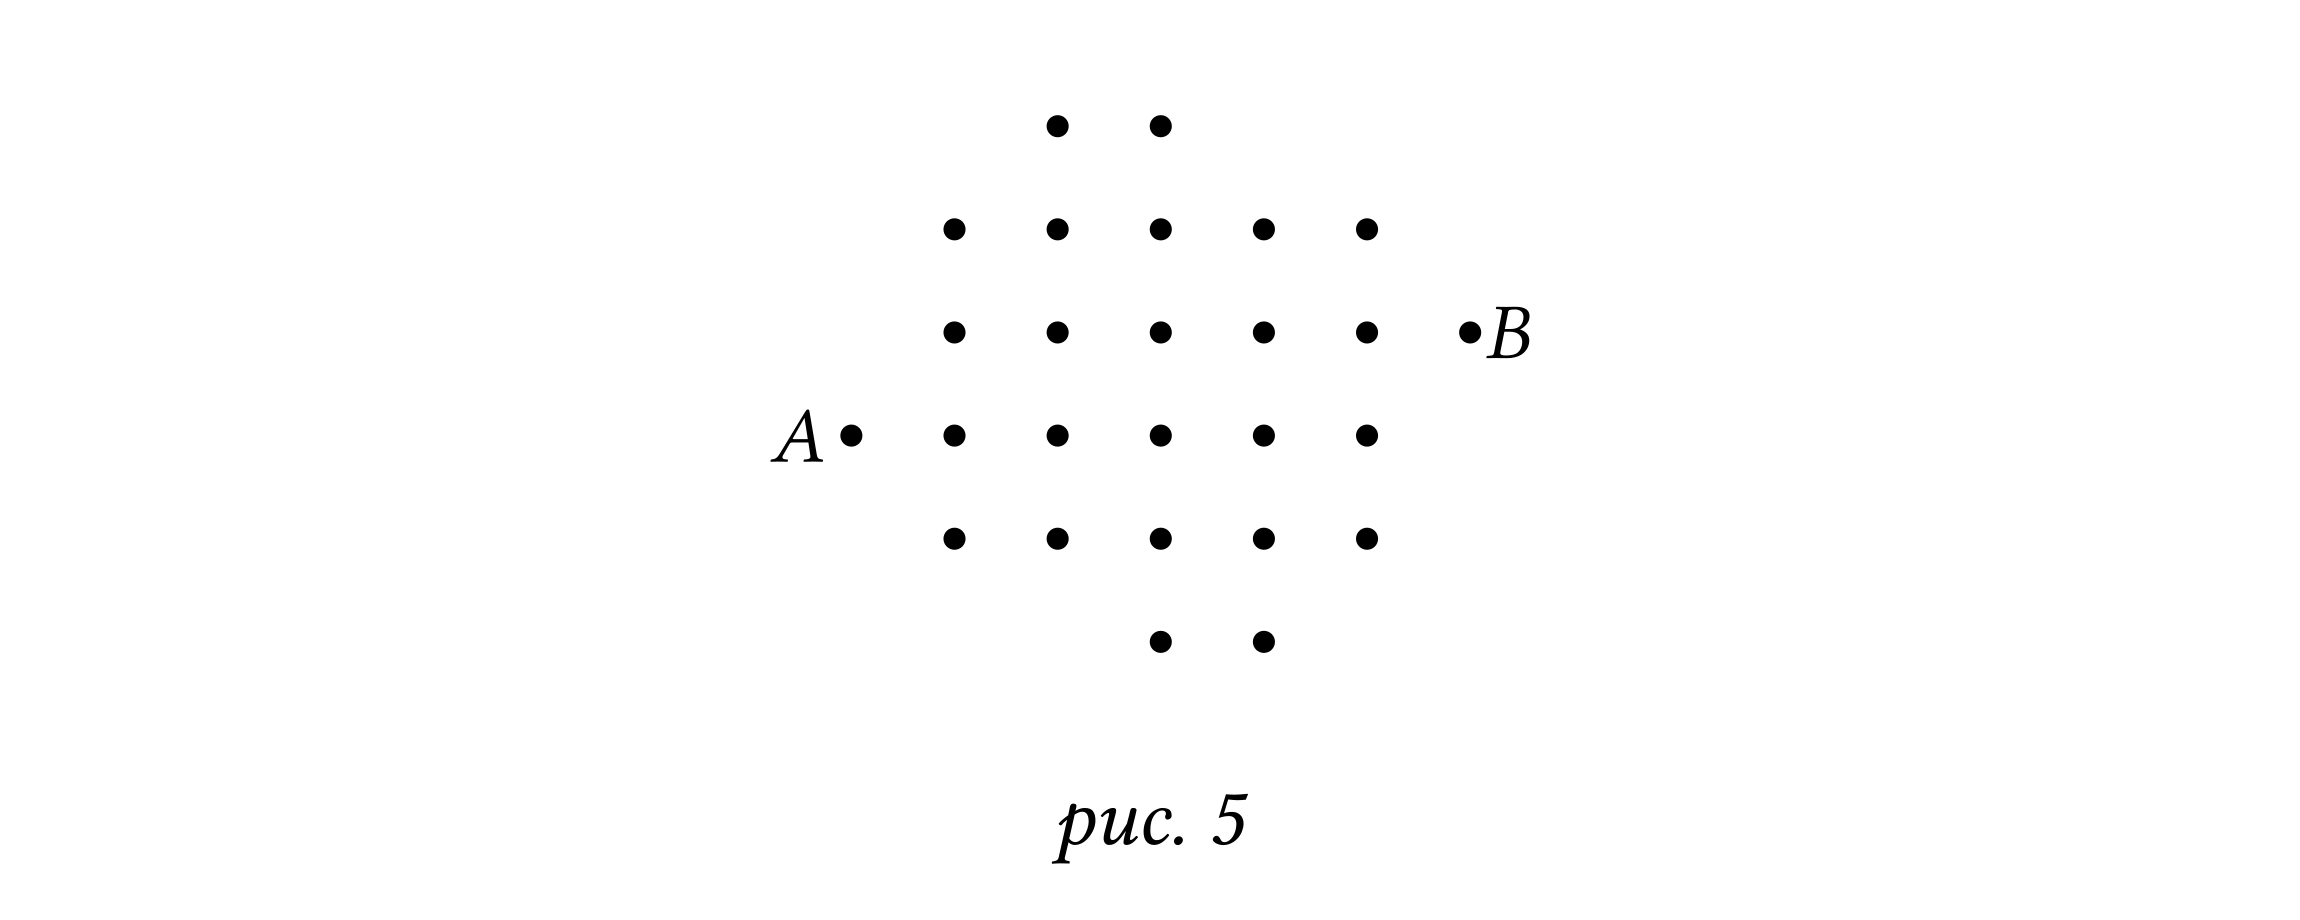
\includegraphics[width=10cm]{stats/2016/Figures/Gvozdiks.png}
\end{center}
%%%%%%%%%%%%%%%

%%%%%%%%%%%%%%%
\task{Разделение на подмножества}
\begin{itemize}
\itA Даны две компании из мальчиков, у каждого из которых есть сколько-то денег. Известно, что у любых пяти мальчиков из одной компании денег в сумме столько же, сколько у любых пяти мальчиков из другой компании. Могут ли суммарные количества денег в первой и во второй компаниях различаться?

\itB Петя хочет покрасить единичные отрезки в составе прямой в два цвета так, чтобы среди любых четырёх подряд идущих отрезков было ровно два чёрных, а среди любых одиннадцати подряд идущих — ровно шесть чёрных. Может ли он это сделать?

\itC На клетчатой бумаге водятся четыре вида муравьёв, ареал каждого представляет собой связное множество клеток. Ареалы разных видов могут пересекаться. Сколько возможных комбинаций видов муравьёв может жить в клетке? Изобразите ареалы видов муравьёв такие, что каждая комбинация видов реализуется хоть на одной клетке.
\end{itemize}
%%%%%%%%%%%%%%%

%%%%%%%%%%%%%%%
\task{Лыжная секция}
\begin{itemize}
\itA Вначале лыжная секция состояла из одного-единственного участника — тренера, но потом в неё каждый день приходило либо 4, либо 5 новых участников. Могло ли в секции после нескольких дней насчитываться ровно 12 участников?

\itB Трое лыжников вышли в лес, чтобы найти хорошее место для новой трассы. Лыжники встали на расстоянии по 100 метров друг от друга. В любой момент времени может двигаться только один лыжник, но при этом лишь по прямой, параллельной отрезку, соединяющему двух оставшихся лыжников. Пару часов покатавшись так по лесу, лыжники замерили расстояние друг между другом — получились цифры в 90, 120 и 150 метров. Докажите, что кто-то из лыжников не выполнял правила в течение поездки.

\itC Из разных точек длинной кольцевой трассы одновременно стартовали 564 лыжника. Во время гонки лыжник мог обогнать другого, но не двоих лыжников сразу. Через некоторое время лыжники одновременно финишировали в тех же точках, из которых стартовали. Могло ли произойти нечётное число обгонов? А если один из лыжников заболел и не явился на старт?
\end{itemize}
%%%%%%%%%%%%%%%

%%%%%%%%%%%%%%%
\task{В поисках чисел}
\begin{itemize}
\itA Составляя условия олимпиады «Математика НОН-СТОП», мальчики Боря и Дима придумывают для участников математические ребусы: выражения, где разным буквам соответствуют разные цифры. Будут ли ребусы \smallskip \\
\centerline{Р$\cdot$О$\cdot$М$\cdot$А$\cdot$Ш$\cdot$К$\cdot$А $=$ РОМАШКА
\ \ \ и\ \ \ 
Я$\cdot$О$\cdot$Т$\cdot$Л$\cdot$И$\cdot$Ч$\cdot$Н$\cdot$И$\cdot$К $=$ УРАУРА} \smallskip
иметь решение?

\itB Вася разбил числа от 3 до 8 включительно на четыре группы. Может ли его друг Рома наверняка утверждать, что произведение чисел в одной из этих групп больше 12?

\itC Для данного числа $n$ предъявите по возможности эффективный алгоритм нахождения 
наименьшего составного числа $N$, такого, 
что $n!$ не делится на $N$, и докажите, что полученное составное число действительно будет 
наименьшим.
\end{itemize}
%%%%%%%%%%%%%%%

%%%%%%%%%%%%%%%
\task{Числа, цифры и приключения}
\begin{itemize}
\itA Девочка Маша открыла в песочнице магазин. Чтобы купить в этом магазине несколько спичек, нужно выложить из них цифру так, как на экране калькулятора, и дать Маше количество листочков, равное этой цифре. Как дешевле всего покупать спички у Маши?

\itB Фирма «DFS» разрабатывает особые космические бульдозеры. Для работы на астероиде под названием Гурбштекен был разработан специальный бульдозер, гусеницы которого делают ровно 953 оборота за 29 проходов по экватору астероида. Для удобства гусеницы бульдозера были разделены на 29 сменных секций, одну из которых пришлось заменить ещё в полёте. Наконец бульдозер принялся ездить вокруг астероида по экватору. Доказать, что вне зависимости от стартового положения гусениц свежеустановленная секция рано или поздно окажется на линии старта. Как часто это будет повторяться?

\itC Вовочка неправильно запомнил доказательство теоремы Евклида. Он думает так: перемножим все простые числа, прибавим к произведению единицу --- и полученное число непременно будет простым. Он хочет воспользоваться этим соображением для поиска простых чисел: перемножить несколько первых простых, прибавить единицу, получить новое простое. Докажите, что таким образом Вовочка всё равно рано или поздно получит составное число.
\end{itemize}

\begin{center}
  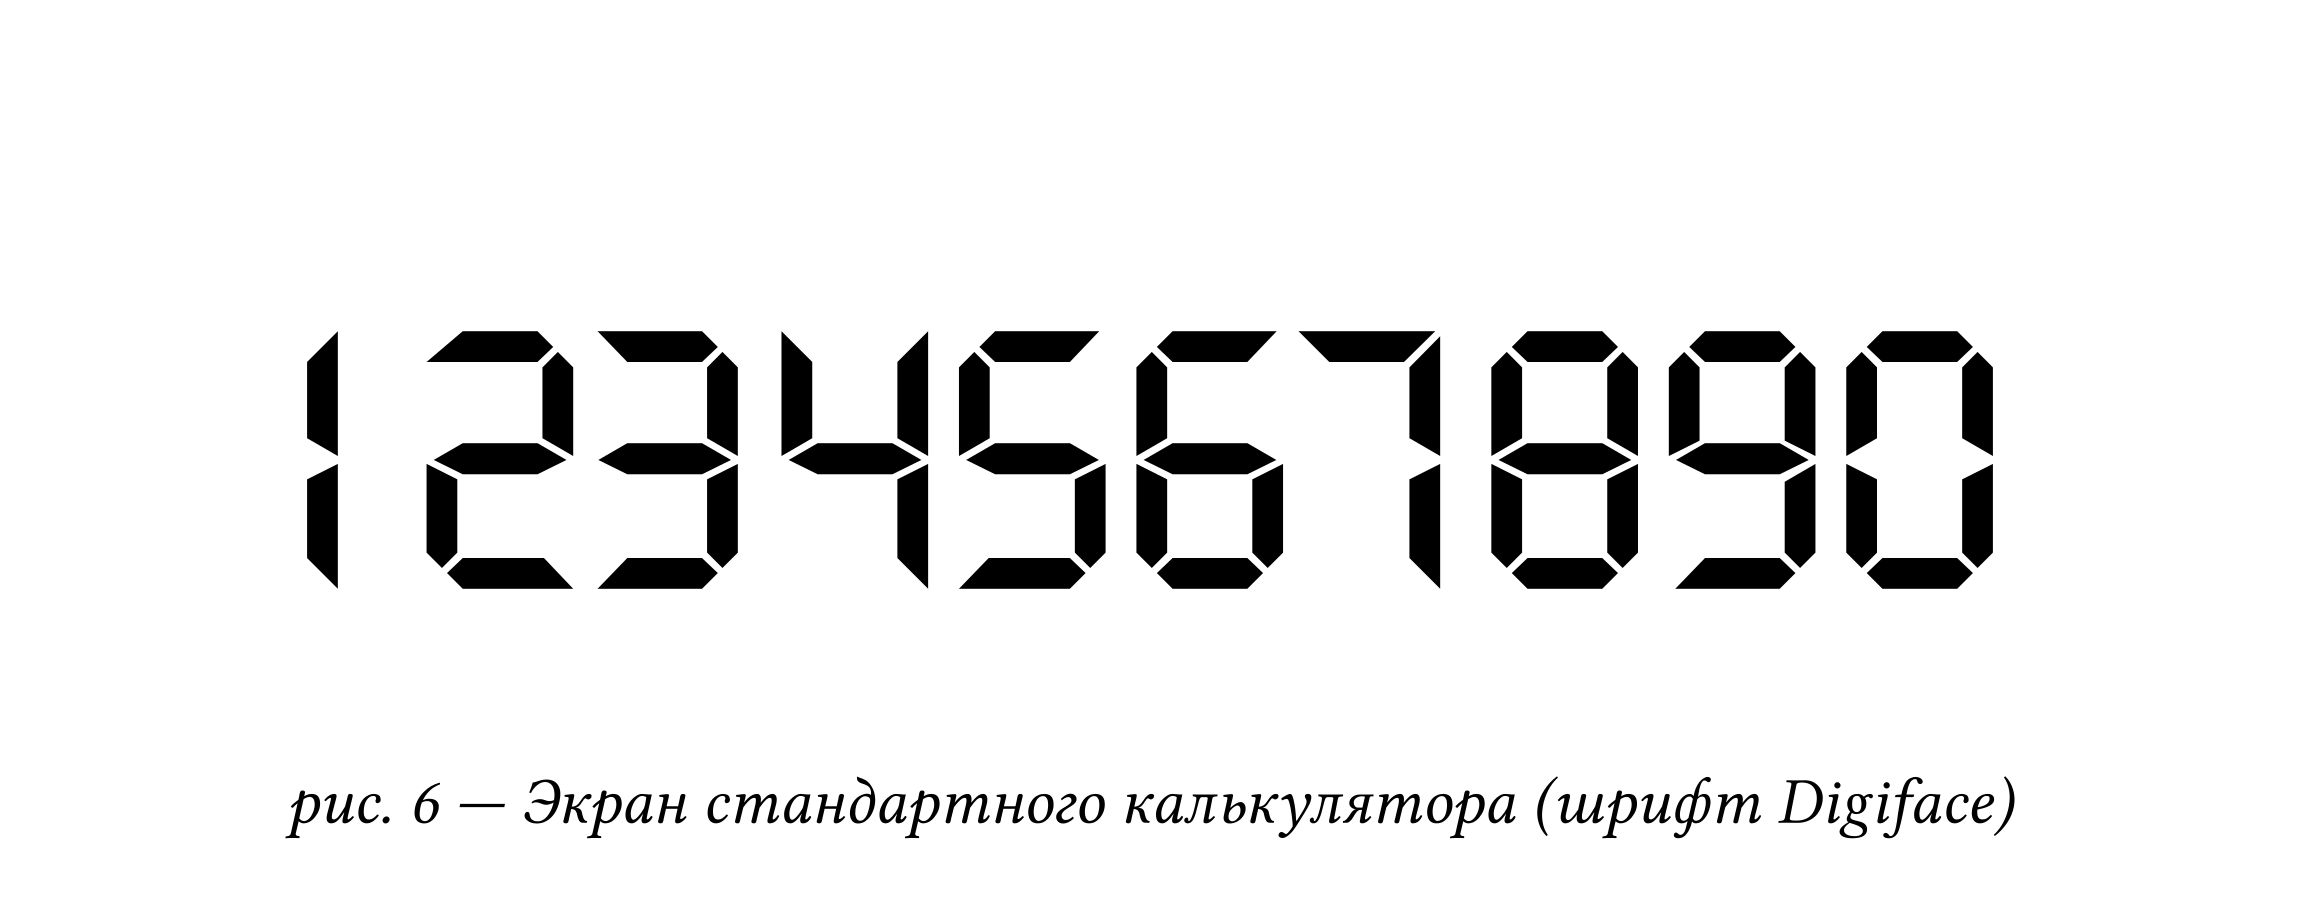
\includegraphics[width=7.5cm]{stats/2016/Figures/Digiface.png}
\end{center}
%%%%%%%%%%%%%%%